\documentclass[a4paper,12pt]{article}

%
%% PACKAGE IMPORTS
%%  If any package needed, import it here
%

\usepackage{styles/ibu-thesis}
\usepackage{subcaption}

%
%% MACROS
%%  If any macro needed, define it here
%
\newcommand{\writecommand}[2]{
    \begin{center}
        \texttt{\textbackslash #1\{\##2\#\}} \\
    \end{center}
}


%
%% THESIS TITLE
%
\thesistitle{Title: \LaTeX~Template for Project}

%
%% AUTHOR INFORMATION 
%%  If there is more than 3 author it can be added to list
%%  e.g. \authors[4]{Name of author} and \authorsid[4]{ID of author} etc.
%
\authors[1]{NAME}
\authorsid[1]{ID}
\authors[2]{NAME}
\authorsid[2]{ID}
\authors[3]{NAME}
\authorsid[3]{ID}


%
%% AFFILIATION INFORMATION
%%  Below information are must
%
\assignment{Final Project}
\course{CMPE346: NATURAL LANGUAGE PROCESSING}
\submissiondate{May, 2020}

%
%% ABSTRACT
%%  In case of more than one paragraph abstracts, use \\ separator only 
%%  to open a new paragraph
%%  e.g. ... paragraph ended here. \\ New paragraph starts here ...
%
\abstract{}



\begin{document}

%
%% PRELIMINARIES 
%
\maketitle

\addcontentsline{toc}{section}{\abstractname}
\makeabstract

\addcontentsline{toc}{section}{\contentsname}
\maketableofcontents

\pagenumbering{arabic} % Do not change
\setcounter{page}{1} % Do not change


%
%% SECTIONS
%%  The thesis starts here
%

\section{Sections}
In order to create sections, use \writecommand{section}{Name of Section} command. Every section created will be added to Table of Contents, automatically. 

To reference a section use \writecommand{section}{Name \textbackslash label\{sec:label\}}
command. For detailed information, check Section \ref{sec:in-text-ref}.

\subsection{Subsections}
In order to create subsections, \writecommand{subsection}{Name of Subsection} command. Each \texttt{\textbackslash sub} is added to prefix of command, creates new subsection of previous section. For example, \writecommand{subsubsection}{Name} command will create subsection of a subsection.

\section{Environments}
Each enviroment starts with \writecommand{begin}{name of env} and ends with \writecommand{end}{name of env} Environments allows in-text-referencing. Use \texttt{\textbackslash label} command to label the related environment\footnote{Recommended labeling is using type of environment in label. E.g. \textit{tab:example} for example table.}. Once the environments are labeled, \texttt{\textbackslash ref} command can be used. 

Most of the environments allow silent environments, in case of not referencing in text. This option is provided by \texttt{*} after the name of environments. For example, \texttt{\textbackslash begin \{equation*\}} for silent equations.

\subsection{Equations}
Use \texttt{equation} environment to create your equations. Some examples about equations are given below. Follow \LaTeX~code.

\begin{equation}
    \hat{H} = - \frac{\hbar}{2m}\nabla^2 + \hat{V}(x,y,z)
    \label{eq:hamiltonian}
\end{equation}

Equation \ref{eq:hamiltonian} is used to write a form of the Schrondinger wave function equation in quantum mechanics:

\begin{equation*}
    \hat{H}\psi(x,y,z) = E\psi(x,y,z).
\end{equation*}

Referencing an equation and silent equation examples are given above. Additionally, piece-wise function example are given

\begin{equation}
    \delta_n(x) = 
    \begin{cases}
        0 & x < 0 \\
        ne^{-\pi x} & x > 0
    \end{cases}
\end{equation}


\subsection{Tables}
In order to create tables use \texttt{table} environment. Use \texttt{caption} command for table (or figure) headings. Each table created will be added to Table of Contents, automatically. In order not to use long headings in ToC, short version of the heading can be given with brackets in \texttt{caption} command. See Table \ref{tab:example}.

\begin{table}[h]
    \centering
        \begin{tabular}{r|c c}
         \textbf{Noise} & \textbf{MLP$^*$} & \textbf{BN} \\ \hline 
         $\mu=0$, $\sigma=0$ & 96.6 & 93 \\ 
         $\mu=0$, $\sigma=1$ & 95 & 90.3 \\ 
         $\mu=0$, $\sigma=2$ & 84.6 & 84 \\ 
         $\mu=0$, $\sigma=3$ & 76 & 81.3 \\ 
         $\mu=0$, $\sigma=4$ & 71 & 77.8 \\ 
         $\mu=0$, $\sigma=5$ & 53 & 70.6 \\ 
         $\mu=0$, $\sigma=10$ & 47.3 & 69.3 \\ 
    \end{tabular}
    \caption[Short version of heading for example table]{Lorem ipsum dolor sit amet, consectetur adipiscing elit. Pellentesque non consectetur dui. Integer eget est ipsum. Praesent ultricies venenatis velit, sed porta lorem euismod tincidunt. Suspendisse potenti. Sed eget porttitor sem. Nulla rutrum eleifend enim, quis pharetra nisi placerat nec.}
    \label{tab:example}
\end{table}

Position of table (or figures) can be change by explicitly declaring [h,t,b,p]. Each letter corresponds to \underline{h}ere, \underline{t}op, \underline{b}ottom, and \underline{p}age, respectively.


\subsection{Figures}
In order to create tables use \texttt{table} environment. Use \texttt{caption} command for table (or figure) headings. Each figure created will be added to Table of Contents, automatically. In order not to use long headings in ToC, short version of the heading can be given with brackets in \texttt{caption} command. See Figure \ref{fig:example}.

Figure's size can be adjusted by using options of \texttt{\textbackslash includegraphics} command. See Figure \ref{fig:example}.

\begin{figure}[h]
    \centering
    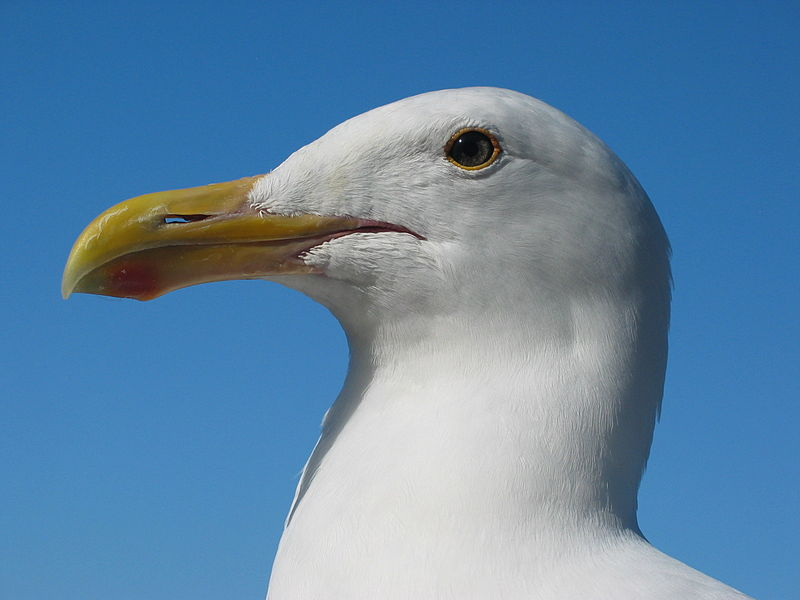
\includegraphics[width=.4\linewidth]{figures/dummy_image.jpg}
    \caption[Short version of heading for example figure]{Lorem ipsum dolor sit amet, consectetur adipiscing elit. Pellentesque non consectetur dui. Integer eget est ipsum. Praesent ultricies venenatis velit, sed porta lorem euismod tincidunt. Suspendisse potenti. Sed eget porttitor sem. Nulla rutrum eleifend enim, quis pharetra nisi placerat nec.}
    \label{fig:example}
\end{figure}

Figures can be combined by using \texttt{subfigure} environments. See Figure \ref{fig:animals}.

\begin{figure}[h]
    \centering
    \begin{subfigure}{.45\textwidth}
        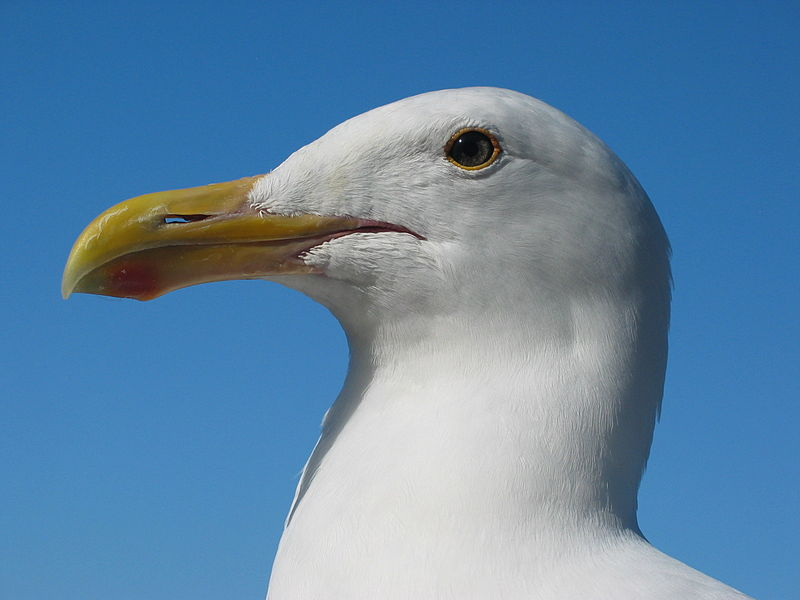
\includegraphics[width=\linewidth]{figures/dummy_image.jpg}
        \caption{Gull image}
        \label{fig:gull}
    \end{subfigure}
    \begin{subfigure}{.45\textwidth}
        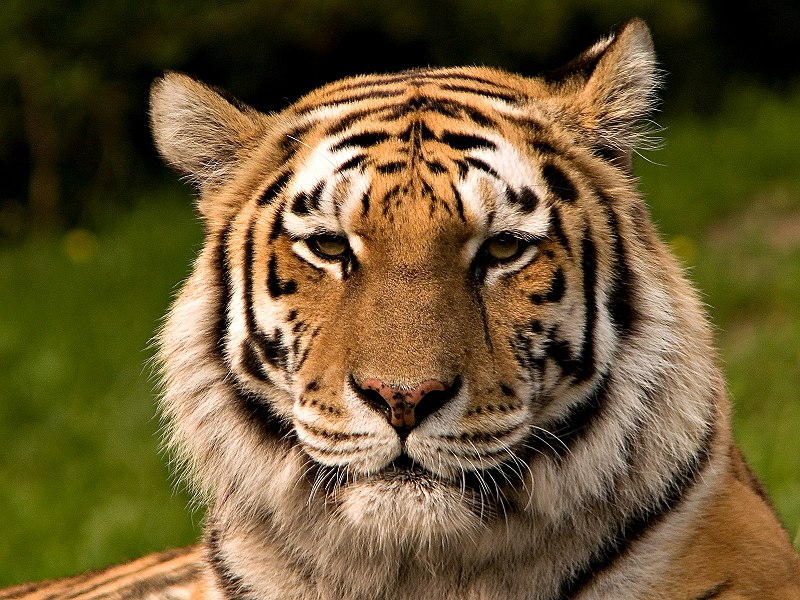
\includegraphics[width=\linewidth]{figures/dummy_image_2.jpg}
        \caption{Tiger image}
        \label{fig:tiger}
    \end{subfigure}
    \caption{Animals}
    \label{fig:animals}
\end{figure}

\subsection{Algorithms}
In order to provide algorithms \texttt{\textbackslash algorithm} environment can be used. See Algorithm \ref{alg:example}.

\begin{algorithm}[h]
    \caption{Finding path from reward matrix}\label{alg:example}
    \begin{algorithmic}[1]
        \Function{Find\_Path}{}
            \While {$i \gets last\_step \text{ to } 0$} \Comment{Bottom-up}
                \State $\textsc{Path}[i] = \textsc{Find\_Argmax}(R[i],\textsc{Path}[i+1])$
            \EndWhile
        \EndFunction
        \State
        \Function{Find\_Argmax}{r[\ ], curr}
            \State $argmax, tmp \gets 0$
            \For {$i \gets 0 \text{ to M*N-1} $} \Comment{Son oda hariç tüm odalar}
                \If {$\text{r[i]} > tmp \text{ and } \textsc{Is\_Neighbor}(i, curr) $}
                    \State $tmp \gets \text{r[i]}$
                    \State $argmax \gets i$
                \EndIf  
            \EndFor
            \State \Return $argmax$
        \EndFunction
    \end{algorithmic}
\end{algorithm}

Alternative to \texttt{algorithm} package, \texttt{lstlisting} package can be used. See Code \ref{code:example}.

\begin{lstlisting}[language=Python, caption=An listing example, label={code:example}]
def naive_bayes_predict(query, likelihood):
    posterior = {'neutral': 1, 'insult': 1}

    # P(A|q) = P(A) * [P(w_0|A) * P(w_1|A) * ... * P(w_q|A)]
    for word in query:
        posterior['neutral'] *= likelihood[word]['neutral']
        posterior['insult'] *= likelihood[word]['insult']

    posterior['neutral'] *= likelihood['p_neutral'] # P(A)
    posterior['insult'] *= likelihood['p_insult'] # P(B)

    # Predict class with max posterior
    return np.argmax(list(posterior.values()))
\end{lstlisting}


\subsection{Itemize and Enumerate}
Itemize (or enumerate) environments can support your writings. An example of \textit{itemize} environment given below.

\begin{itemize}
    \item Item 1
    \item Item 2
\end{itemize}

Also both environments support create sub-items as given below.

\begin{enumerate}
    \item Item 1
    \begin{enumerate}
        \item Item in item
    \end{enumerate}
    \item Item 2
\end{enumerate}


\subsection{Footnote}
In order to provide footnotes \writecommand{footnote}{Footnote message} command is used. For including link in footnote, \texttt{\textbackslash url}\footnote{\url{https://www.bilgi.edu.tr/en/}} or \texttt{\textbackslash href}\footnote{\href{https://www.bilgi.edu.tr/en/}{Istanbul Bilgi University Website}} commands can be used.


\section{Referencing}

\subsection{In Text Referencing \label{sec:in-text-ref}}
In order to provide in-text referencing \writecommand{ref}{Label of reference} is used. For better text formatting, it'd better to provide type of the environment as well, e.g. Figure \ref{fig:animals} or Equation \ref{eq:hamiltonian}.

\subsection{Bibliography}

In order to reference another paper in your text, use \writecommand{cite}{Label of bibitem} For example, 
\\[1\baselineskip]
\indent\textit{Alan Turing is one of the founders of Artificial Intelligence domain by questioning whether machines can think or not.\cite{turing2009computing}} \\[1\baselineskip] 
There is two options to manage bibliography in the papers. Be careful that these options are for individual usage, blending two option is not allowed. 

\subsubsection{Using BibTeX File}
BibTeX is an easy-to-use tool for managing the bibliography in papers. BibTeX format of citations\footnote{Google Scholar is recommended source to find BibTeX cite of the papers.} need to be added to a \texttt{.bib} file. A sample of bibliography is given in \texttt{sample.bib} file. Once the bibliography is completed, use \writecommand{bibliography}{Name of BibTeX file} command to add references to the paper.

\subsubsection{Creating Own Bibliography}
Another option to use BibTeX, you can create and manage your own bibliography. In order to create bibliography use \texttt{thebibliography} environment; to add an citation, use
\begin{center}
    \texttt{\textbackslash bibitem\{\#Label of Citation\#\}\{\#Citation Text\#\}} \\
\end{center}
command. Check \LaTeX~code, for further examples. 



%
%% BIBLIOGRAPHY
%
\clearpage
\bibliographystyle{ieeetr}
\addcontentsline{toc}{section}{References}

%
%% USING .bib FILE
%
\bibliography{sample}

%
%% CREATING OWN BIBLIOGRAPHY
%

% \begin{thebibliography}{100}
% \bibitem{turing2009}{Turing, Alan M. "Computing machinery and intelligence." Parsing the Turing Test. Springer, Dordrecht, 2009. 23-65.}
% \bibitem{einstein1905} Albert Einstein. \textit{Zur Elektrodynamik bewegter K{\"o}rper}. (German) [\textit{On the electrodynamics of moving bodies}]. Annalen der Physik, 322(10):891–921, 1905.
% \end{thebibliography}


\end{document}
